\section{Comparison}

Table \ref{tab:fluid_comparison} shows a summary of the comparison of the five fluid simulation methods.

\begin{table}[!htbp]
\centering
\caption{Comparison of Fluid Simulation Methods}
\label{tab:fluid_comparison}
\begin{tabularx}{\columnwidth}{l X X}
\toprule
\textbf{Method} & \textbf{Pro} & \textbf{Con} \\
\midrule
Grid&
Fast (real-time) \newline
Unconditionally stable &
Loss of detail \newline
Not physically accurate \\
\midrule
Particle&
Fast &
Limitation of input particle position \newline
Particle collapse \\
\midrule
PIC&
Stable &
High numerical dissipation \newline
Particles lose energy quickly \\
\midrule
PIC/FLIP &
More realistic and dynamic motion &
Less stable \newline
Needs tuning \\
\midrule
APIC &
Preserves rotation &
More complex \newline
Slower \\
\bottomrule
\end{tabularx}
\end{table}

\subsection{Grid}

We evaluated the performance of the Grid method with a 50x50 grid. Figure~\ref{fig:grid} shows simulation snapshots of the grid simulation.

\begin{figure*}[h]
    \centering
    \begin{subfigure}[b]{0.2\textwidth}
        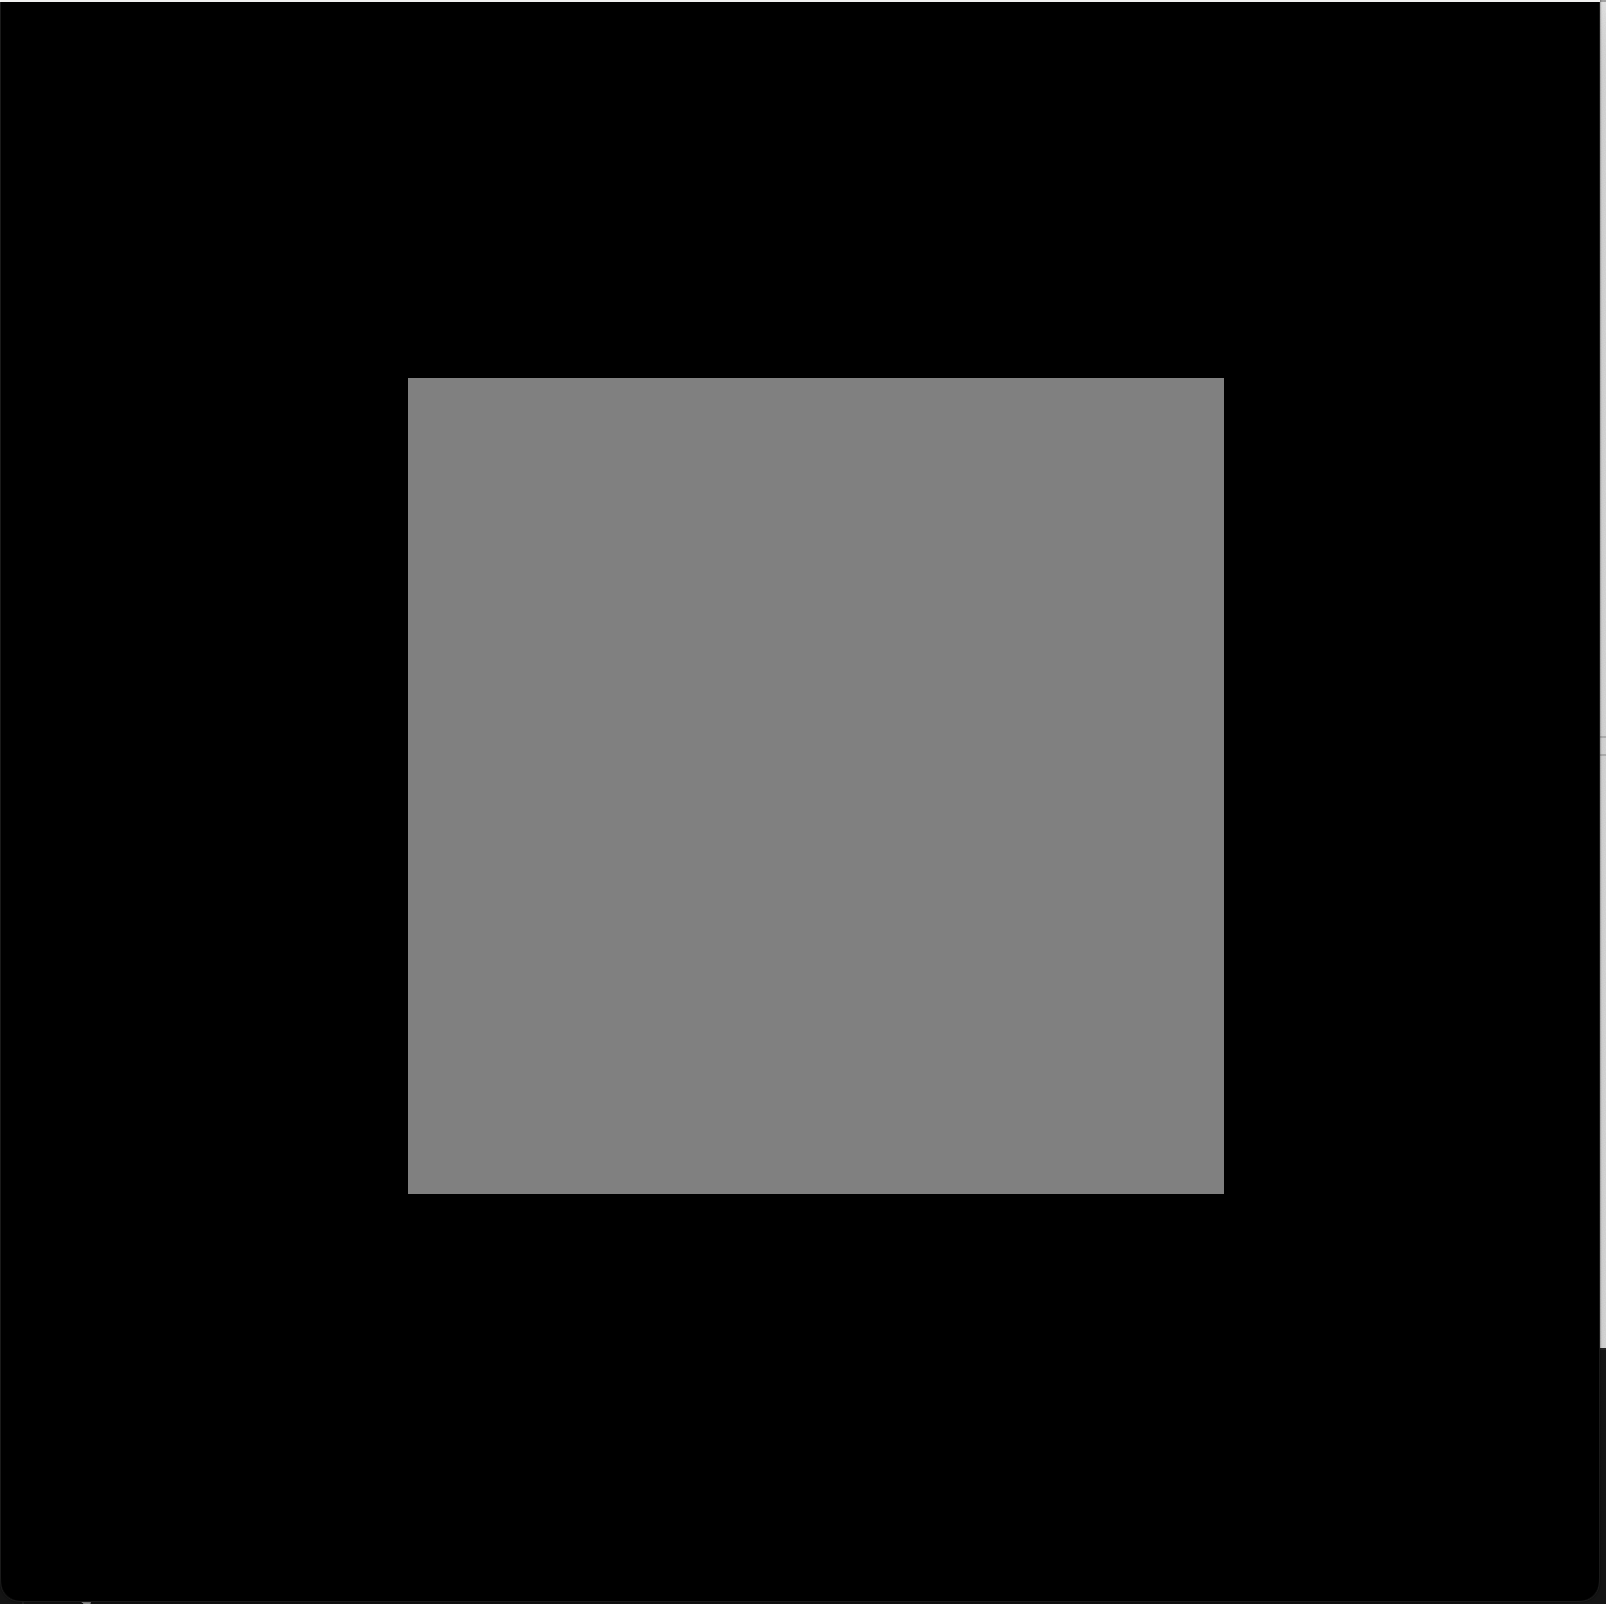
\includegraphics[width=\textwidth]{figures/grid50_init.png}
        \caption{initialization}
    \end{subfigure}
    \hspace{1em}
    \begin{subfigure}[b]{0.2\textwidth}
        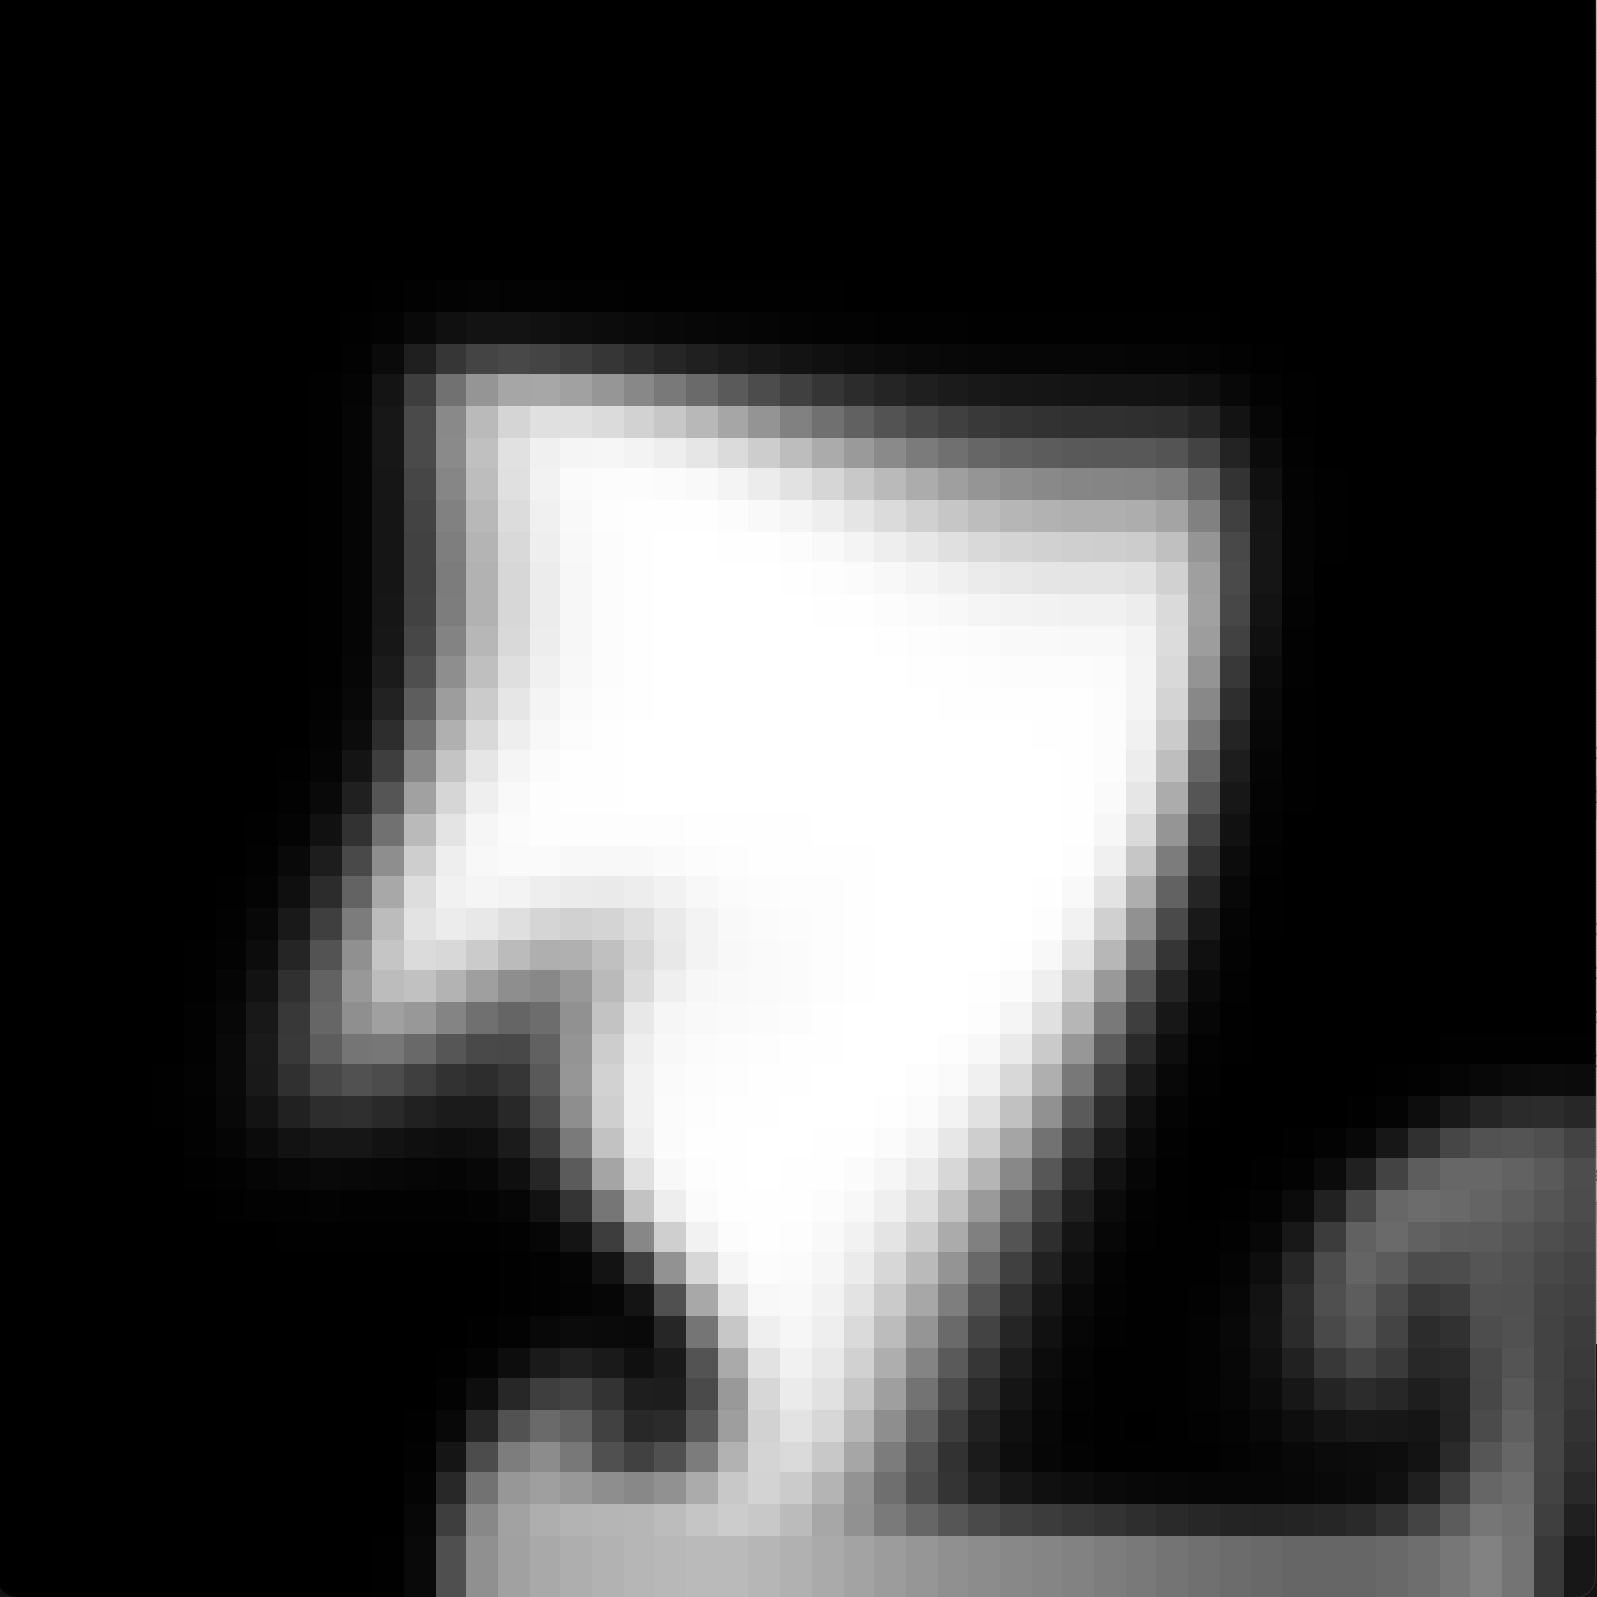
\includegraphics[width=\textwidth]{figures/grid50_1.png}
        \caption{first stage}
    \end{subfigure}
    \hspace{1em}
    \begin{subfigure}[b]{0.2\textwidth}
        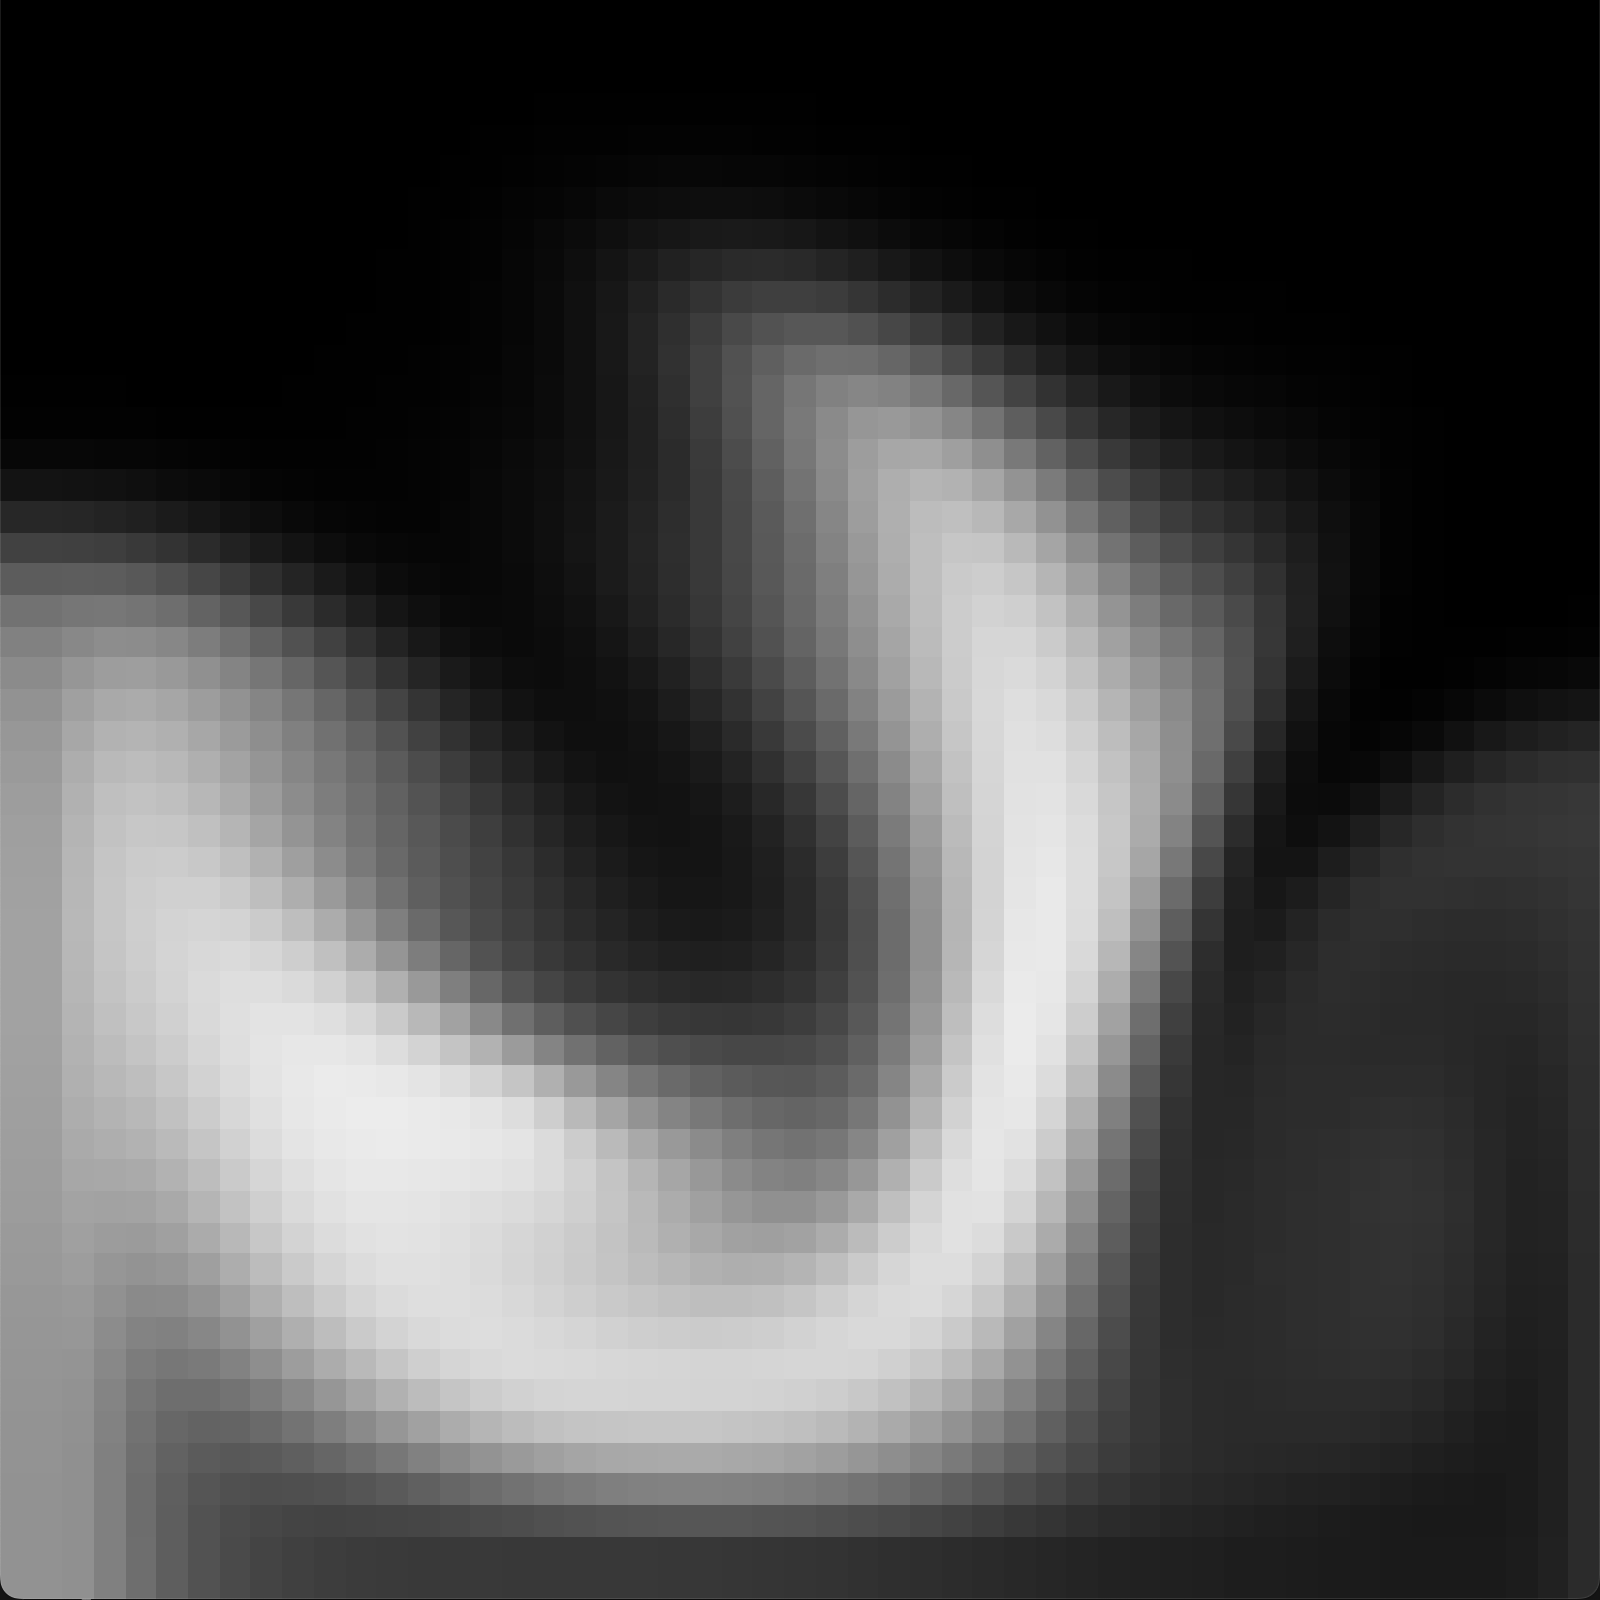
\includegraphics[width=\textwidth]{figures/grid50_2.png}
        \caption{second stage}
    \end{subfigure}
    \hspace{1em}
    \begin{subfigure}[b]{0.2\textwidth}
        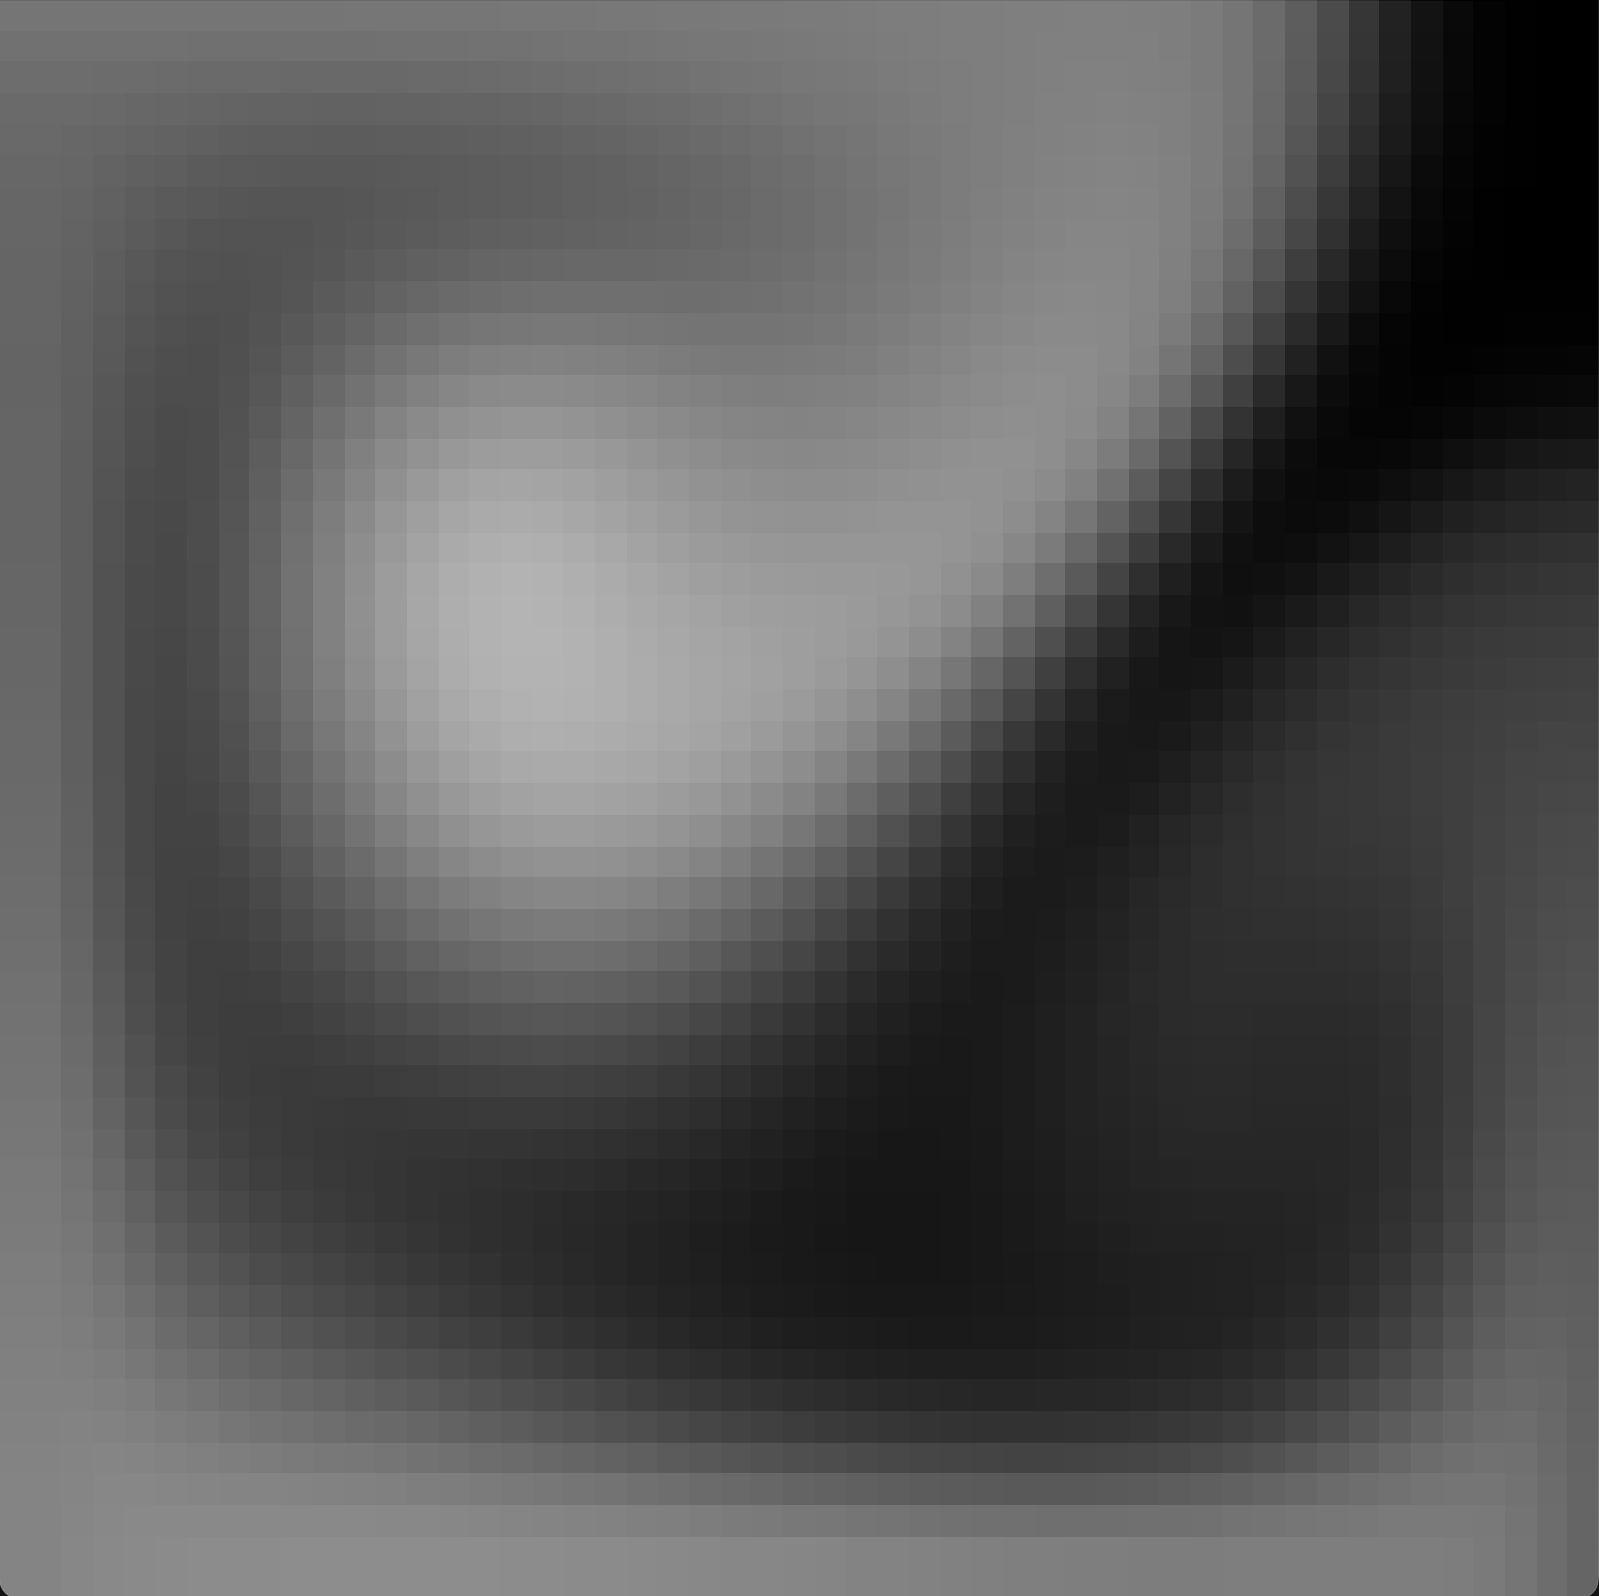
\includegraphics[width=\textwidth]{figures/grid50_3.png}
        \caption{third stage}
    \end{subfigure}
    \caption{Stages of Stable Fluids simulation on a 50x50 grid
    (a) shows the initial grid configuration
    (b)–(d) show different stages of the simulation}
    \label{fig:grid}
\end{figure*}

\subsection{Particle}
Smoothed Particle Hydrodynamics (SPH) contributed to a fast and scalable fluid simulation. The method is more intuitive, and can be used to model free surfaces, avoiding issues that are present in grid simulation such as grid aliasing.
Compared to Stable Fluids, SPH is less stable, and can lead to particle clumping if not stabilized. When initializing the particles, the method is sensitive to particle distribution and requires attention to tuning the smoothing kernels.

\subsection{PIC and PIC/FLIP}

In the Figure~\ref{fig:pic}, the \textbf{yellow arrows} show the grid velocity at some grid points.

\begin{figure*}[h]
  \centering
  \begin{subfigure}[t]{0.2\textwidth}
      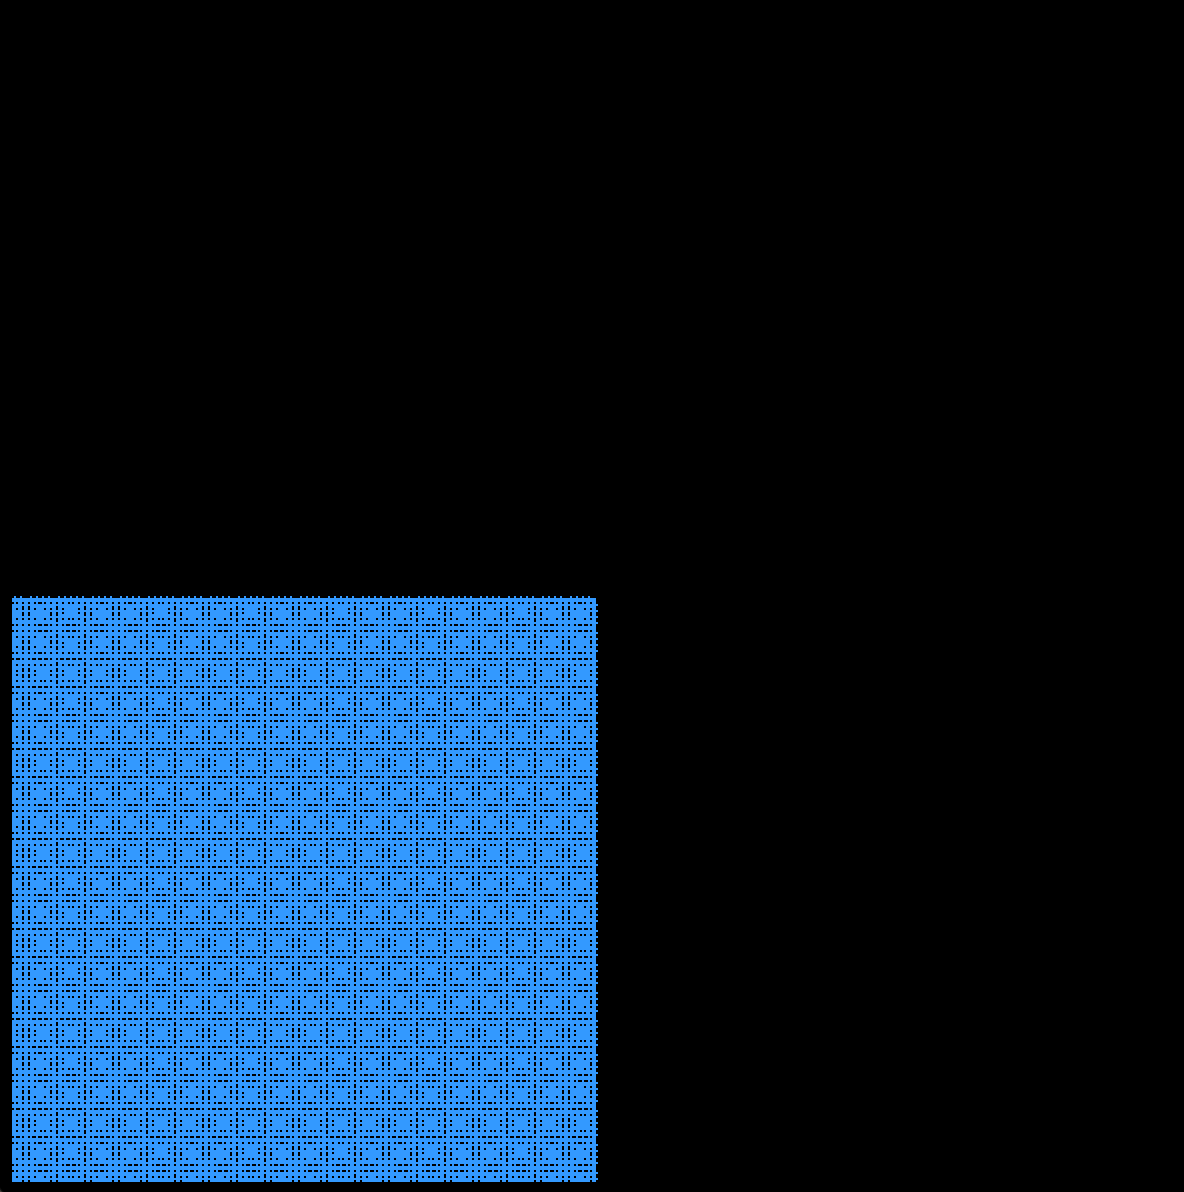
\includegraphics[width=\textwidth]{figures/pic_init.png}
      \caption{Initially, all particles are in the bottom-left corner.}
  \end{subfigure}
  \hspace{1em}
  \begin{subfigure}[t]{0.2\textwidth}
      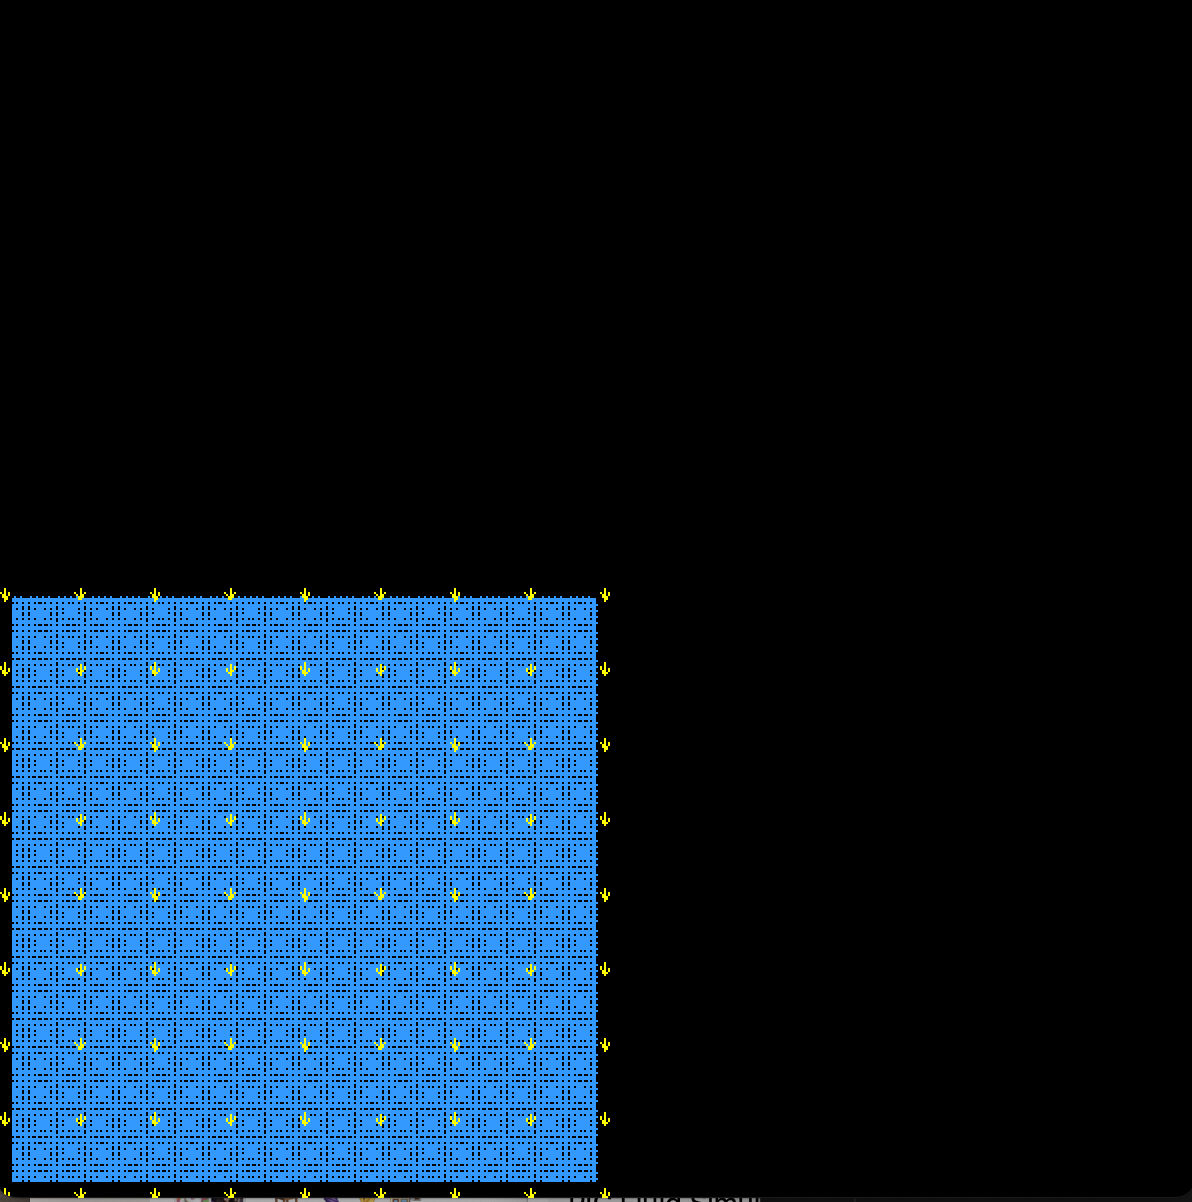
\includegraphics[width=\textwidth]{figures/pic_apply_g.png}
      \caption{After gravity is added, the grid velocity points downward.}
  \end{subfigure}
  \hspace{1em}
  \begin{subfigure}[t]{0.2\textwidth}
    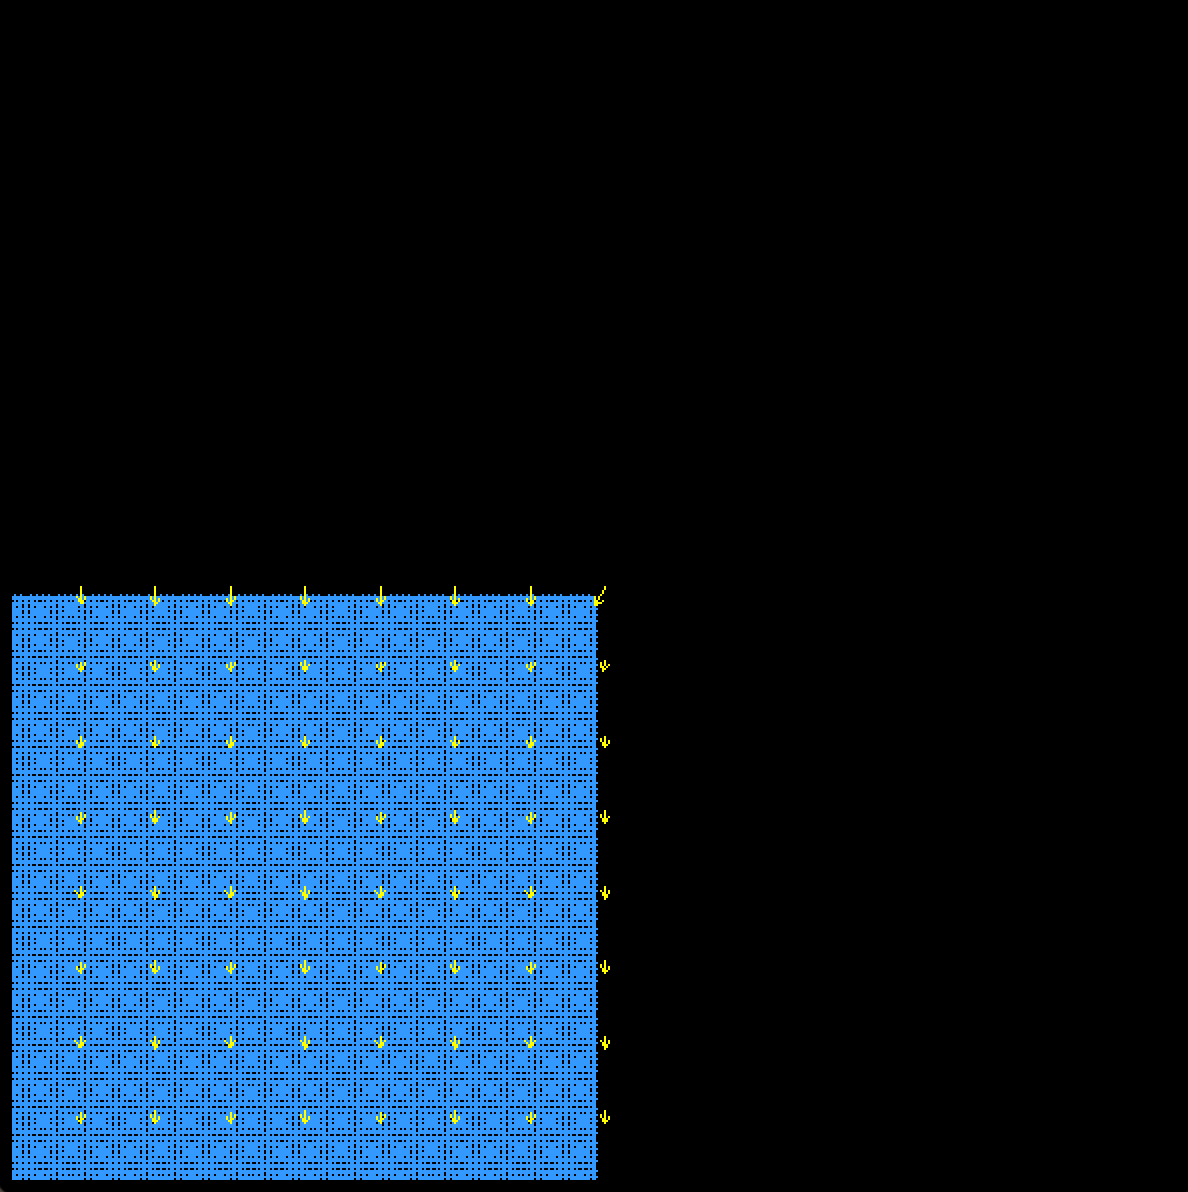
\includegraphics[width=\textwidth]{figures/pic_solve_pr.png}
    \caption{After solving pressure, the grid velocity becomes balanced.}
  \end{subfigure}
  \hspace{1em}
  \begin{subfigure}[t]{0.2\textwidth}
    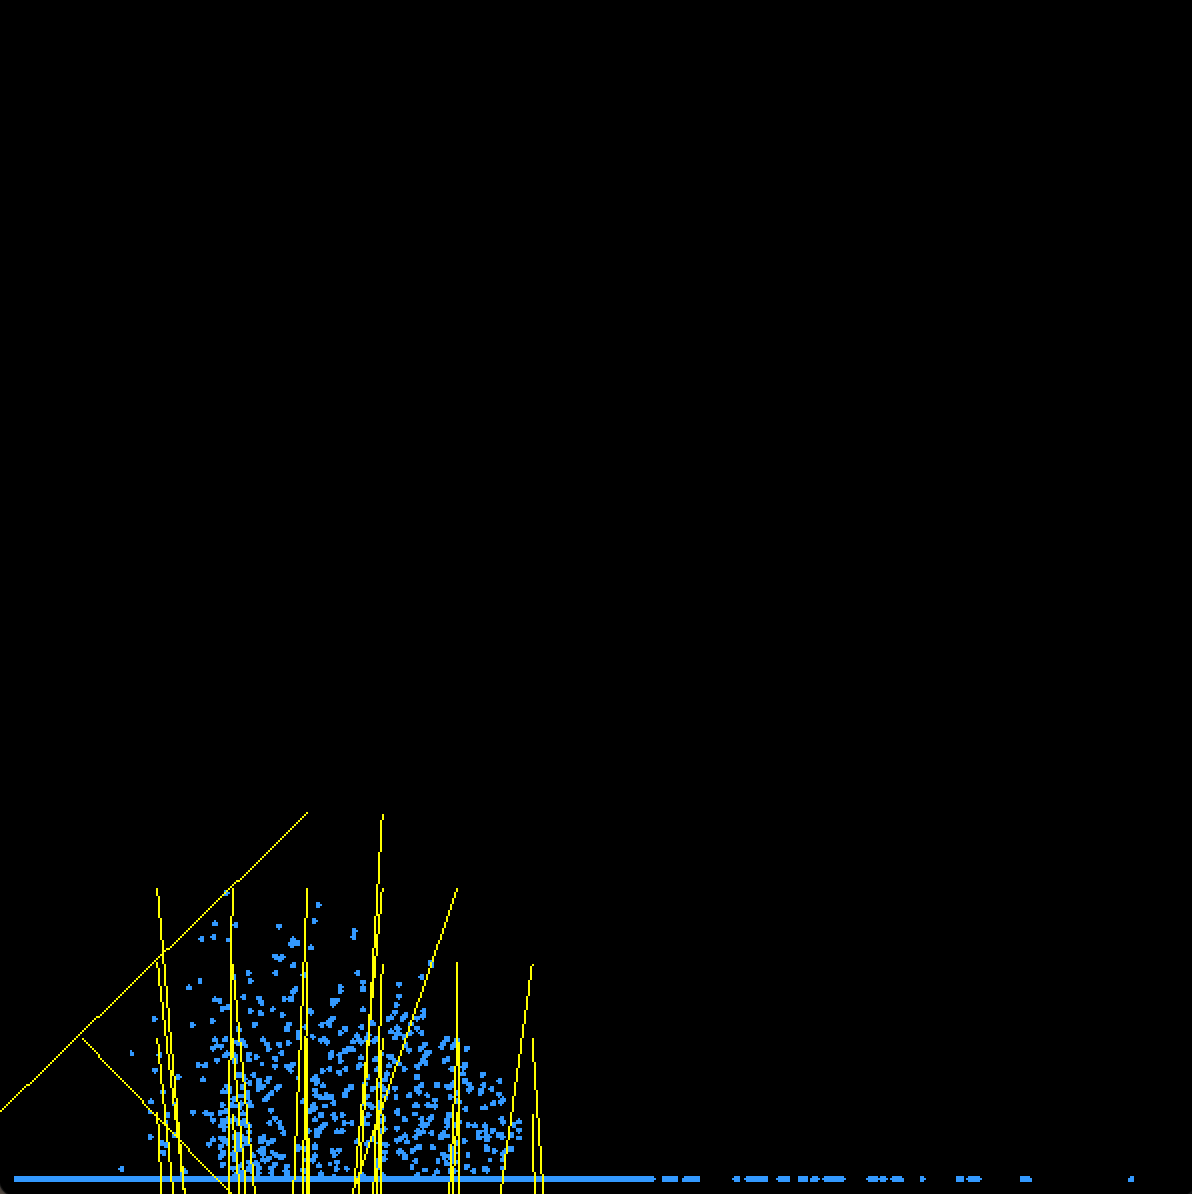
\includegraphics[width=\textwidth]{figures/pic_interm.png}
    \caption{Particles start to move after updating their velocity.}
  \end{subfigure}
  \caption{PIC simulation: Grid velocities update loop}
  \label{fig:pic}
\end{figure*}

We tested both the PIC and PIC/FLIP methods with the same number of particles. Figure~\ref{fig:pic_comparison} shows how the motion is more dynamic than pure PIC.

The PIC method loses energy fast. Particles move less and quickly fall to the bottom.
The PIC/FLIP method keeps more energy. Particles move more and look more natural.

\begin{figure*}[h]
    \centering
    \begin{subfigure}[t]{0.2\textwidth}
        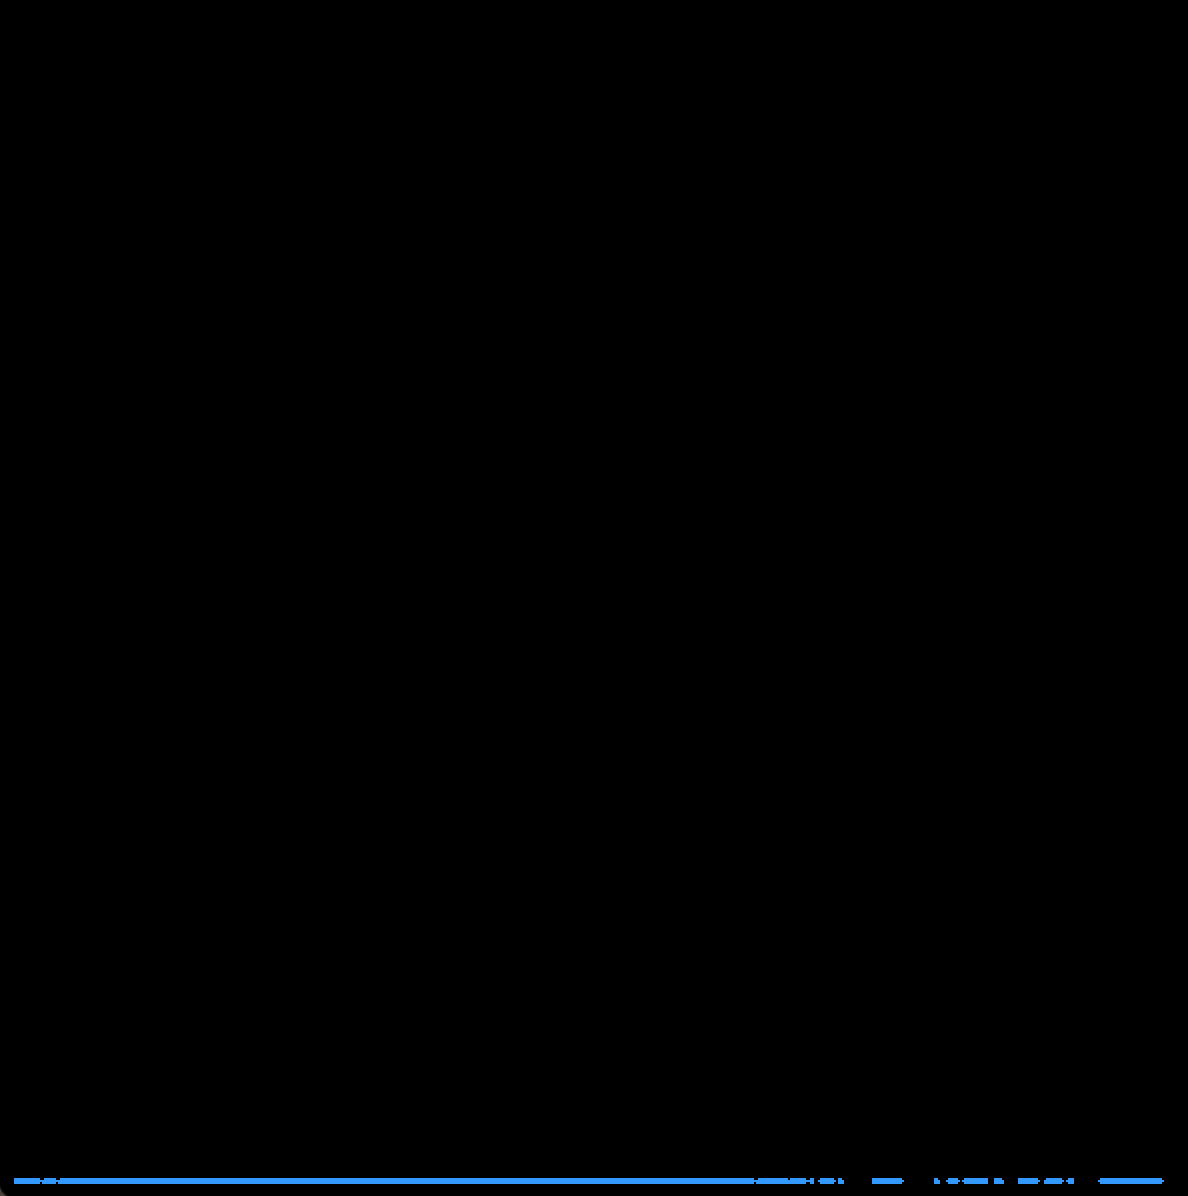
\includegraphics[width=\textwidth]{figures/pic_result.png}
        \caption{PIC result: motion is more damped.}
    \end{subfigure}
    \hspace{1em}
    \begin{subfigure}[t]{0.2\textwidth}
        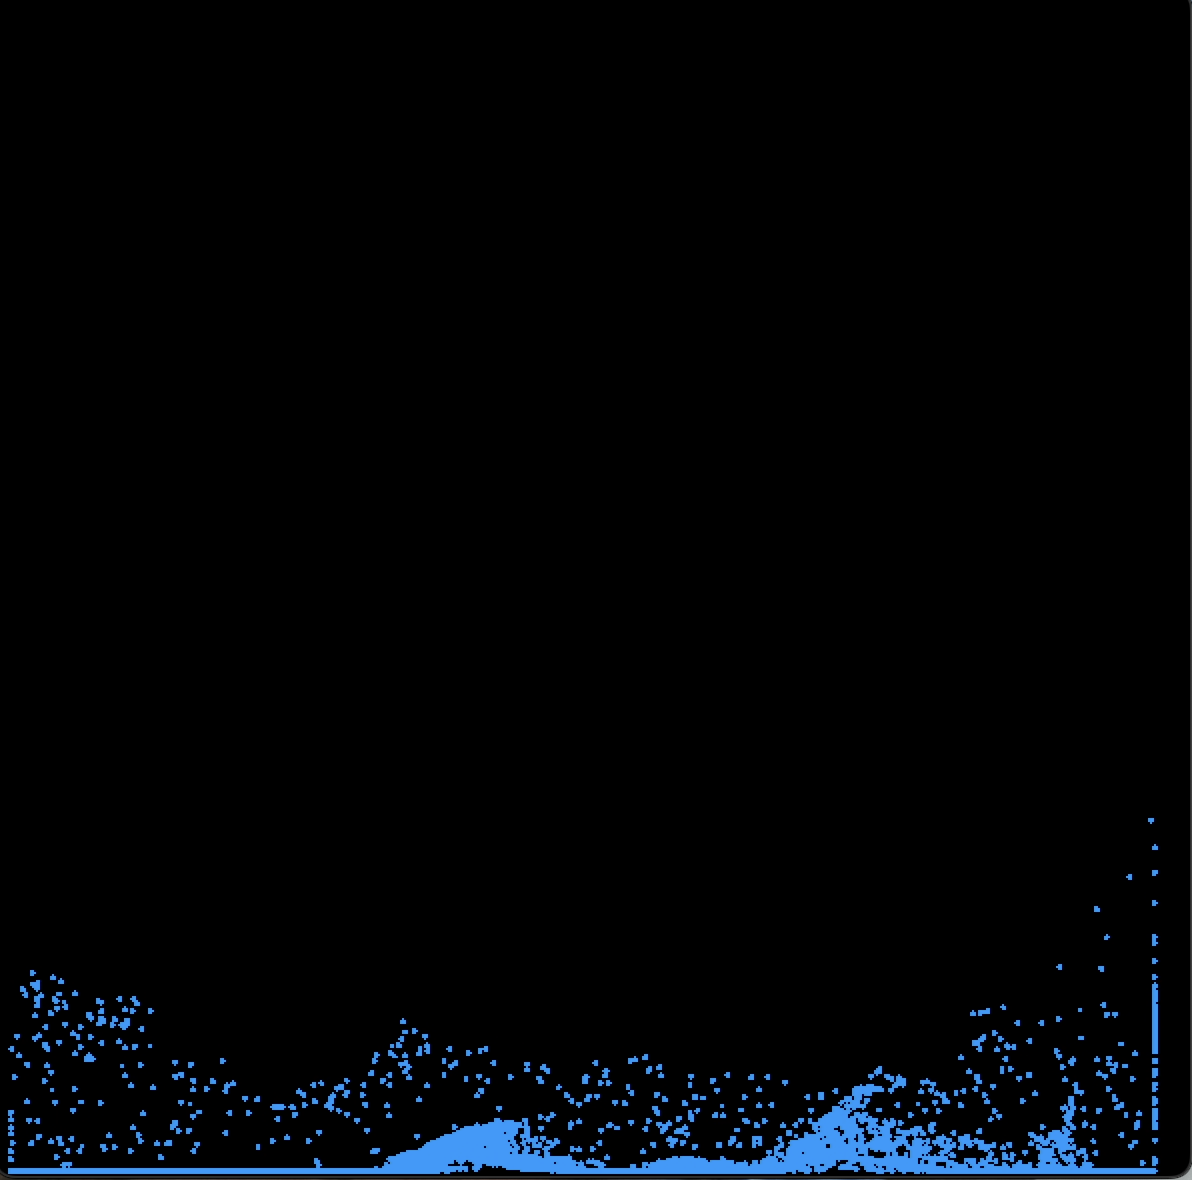
\includegraphics[width=\textwidth]{figures/pic_flip_result.png}
        \caption{PIC/FLIP result: motion is more dynamic.}
    \end{subfigure}
    \hspace{1em}
    \begin{subfigure}[t]{0.2\textwidth}
        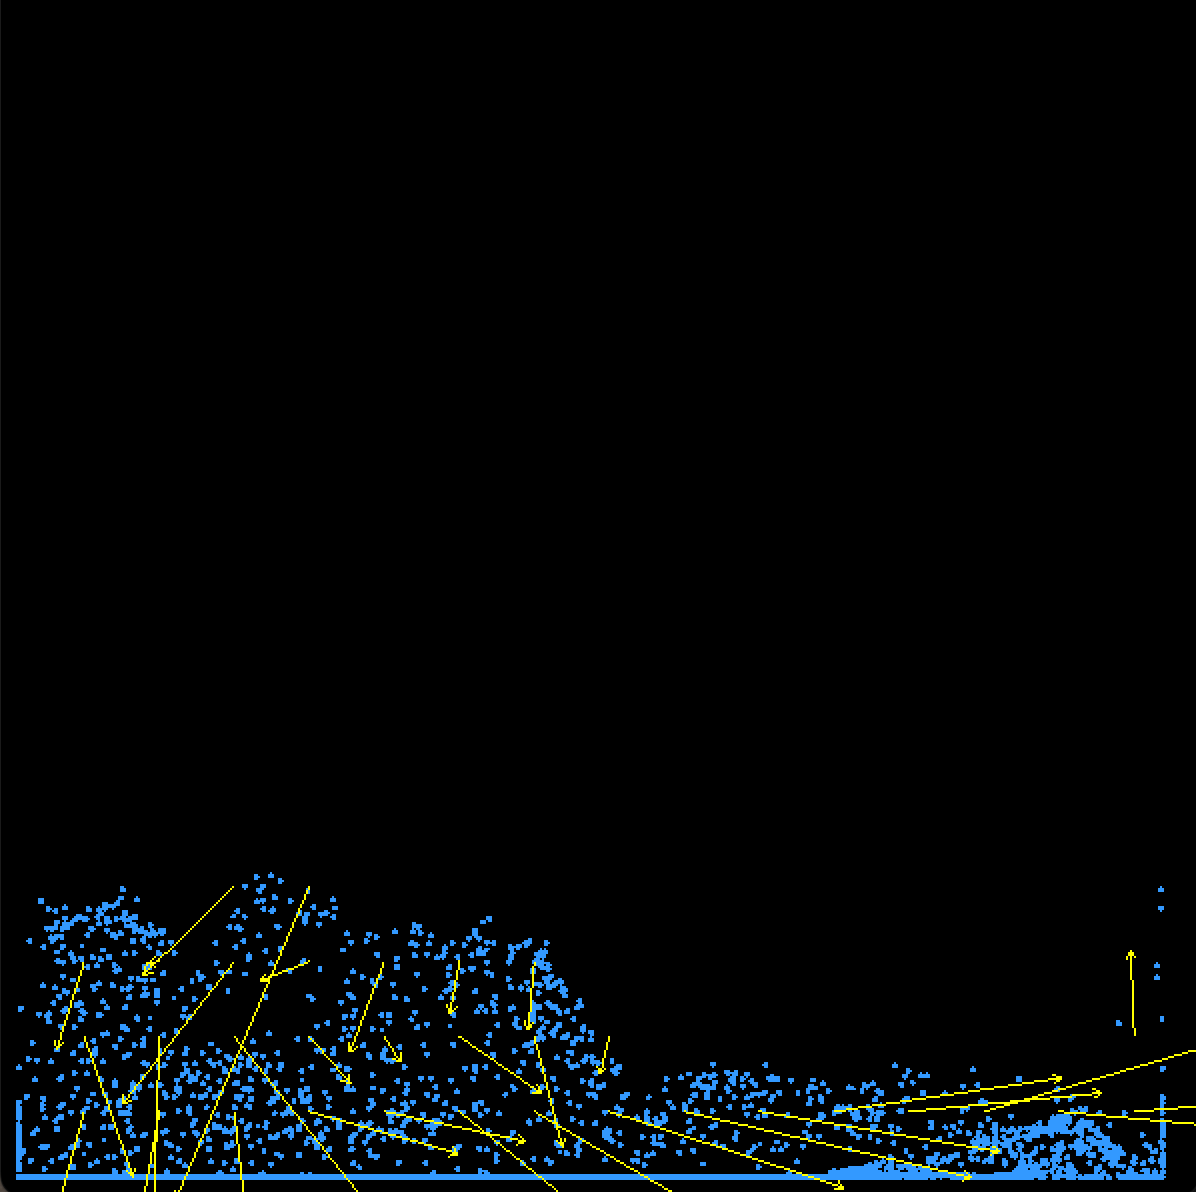
\includegraphics[width=\textwidth]{figures/pic_flip_interm.png}
        \caption{Grid velocities of PIC/FLIP}
    \end{subfigure}
    \caption{Final particle positions using PIC and PIC/FLIP. Both start from the same initial state, but show different behavior due to how velocity is transferred.}
    \label{fig:pic_comparison}
\end{figure*}

\subsection{APIC}
The APIC method contributed most significantly to the visual quality of our simulations. By introducing an affine velocity field per particle, APIC preserves both rotational motion and local deformation, resulting in smoother, more detailed fluid behavior. Compared to PIC and FLIP, it produced the most visually stable and coherent results, especially at higher particle counts. The use of affine velocity transfer also reduced numerical dissipation and prevented particle clumping, leading to more realistic motion.
It is computationally expensive due to affine matrix operations and additional interpolation. Performance drops at high particle counts, and the method becomes less suitable for real-time applications. It is also more complex to implement than PIC or FLIP, requiring careful handling of matrix math, boundary conditions, and velocity transfers to avoid instability.
Figure~\ref{fig:alg:apic_comparison} shows the performance of the APIC method with different particle counts, demonstrating how the method handles fluid detail, stability, and distribution over time.

\begin{figure*}[h]
    \centering
    \begin{subfigure}[b]{0.2\textwidth}
        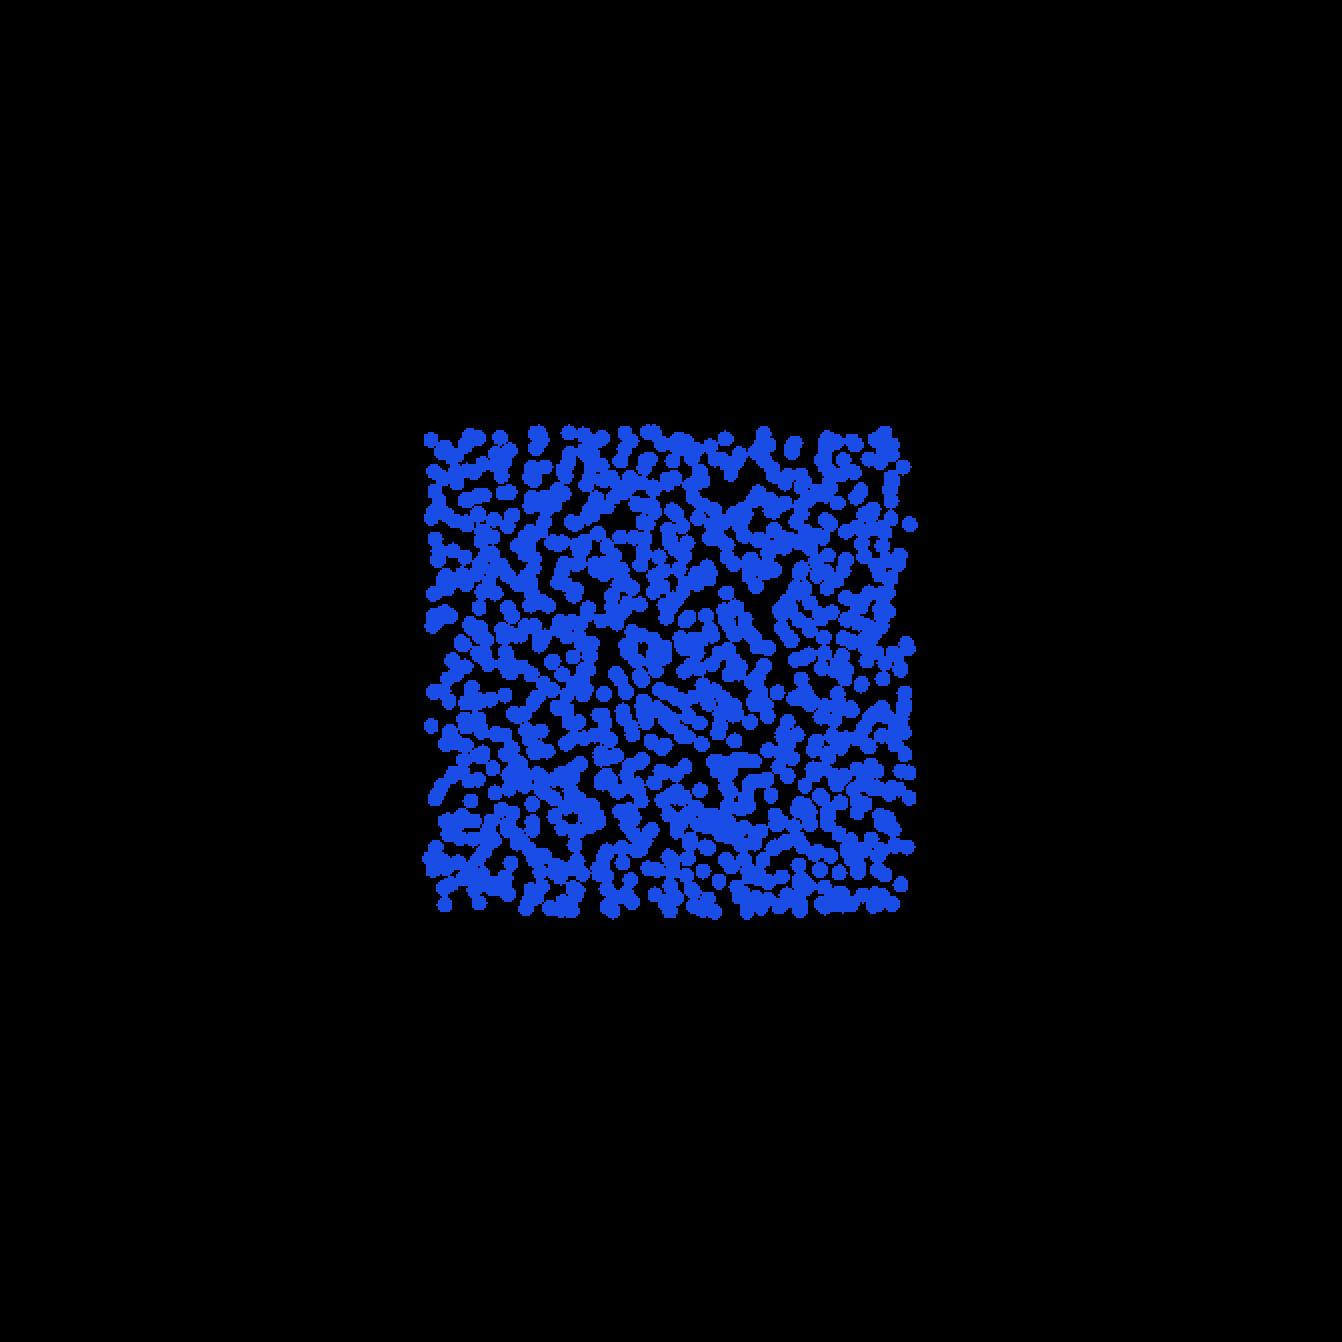
\includegraphics[width=\textwidth]{figures/apic1000_init.png}
        \caption{1000 initial particles}
    \end{subfigure}
    \hspace{1em}
    \begin{subfigure}[b]{0.2\textwidth}
        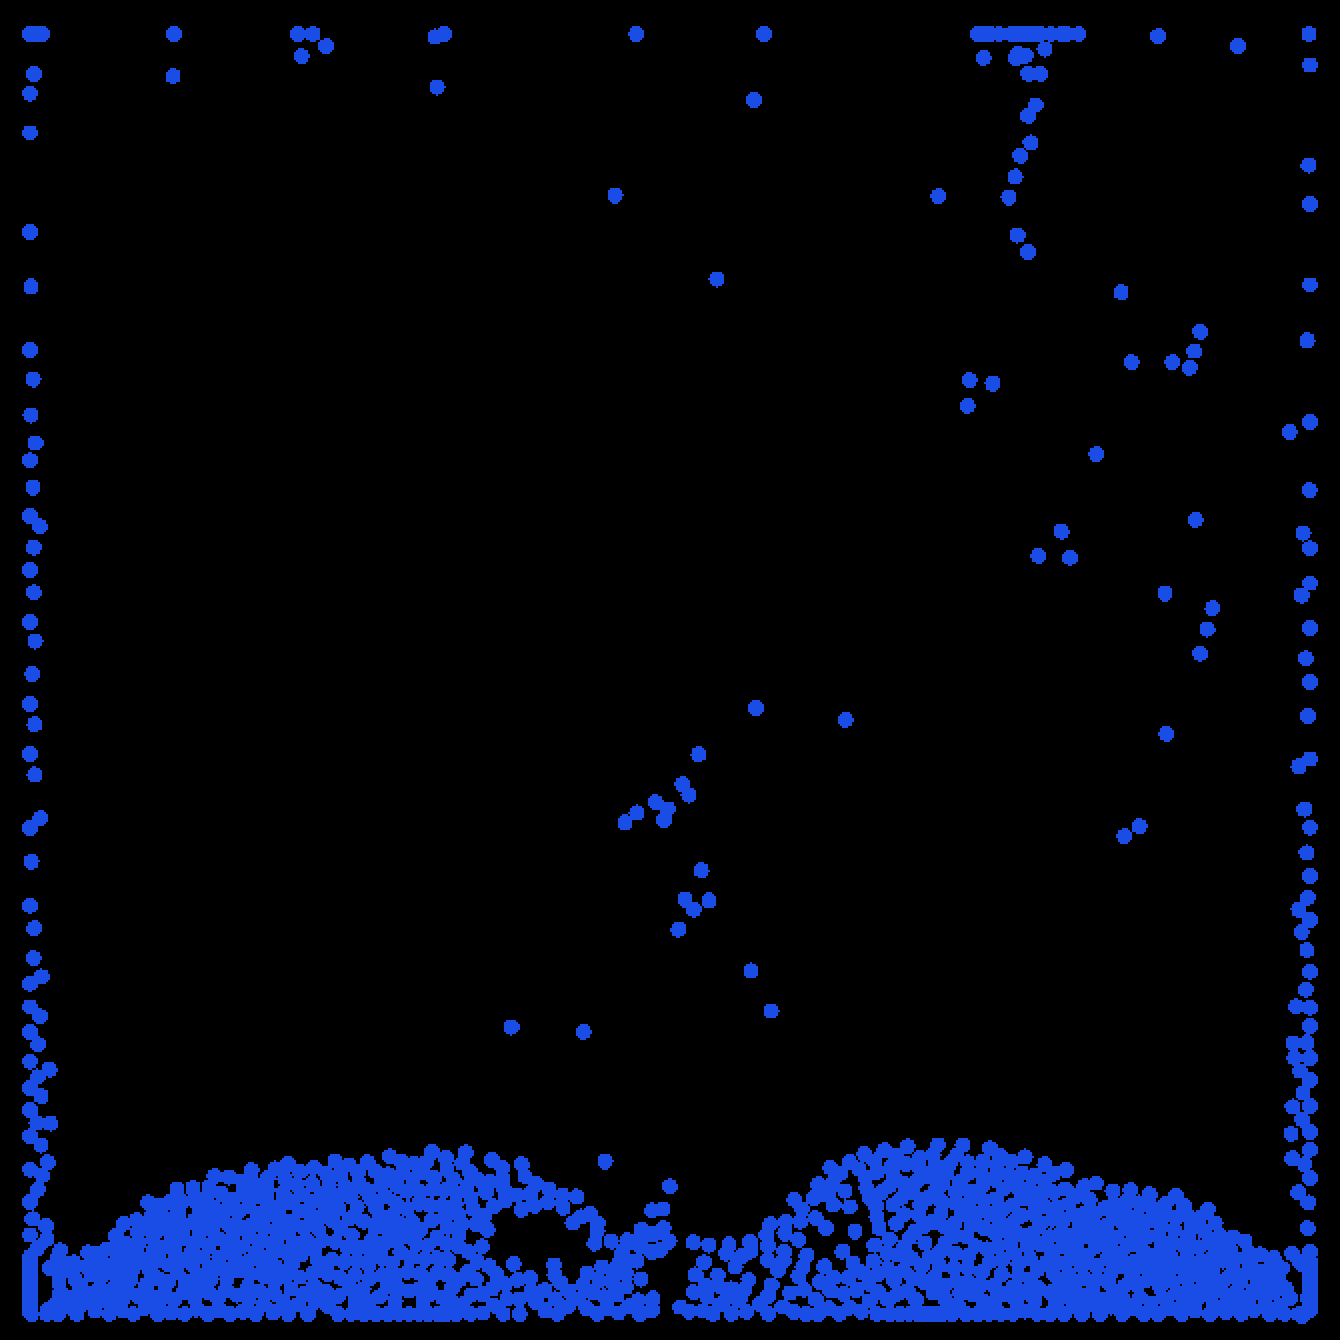
\includegraphics[width=\textwidth]{figures/apic1000.png}
        \caption{1000 particles}
    \end{subfigure}
    \hspace{1em}
    \begin{subfigure}[b]{0.2\textwidth}
        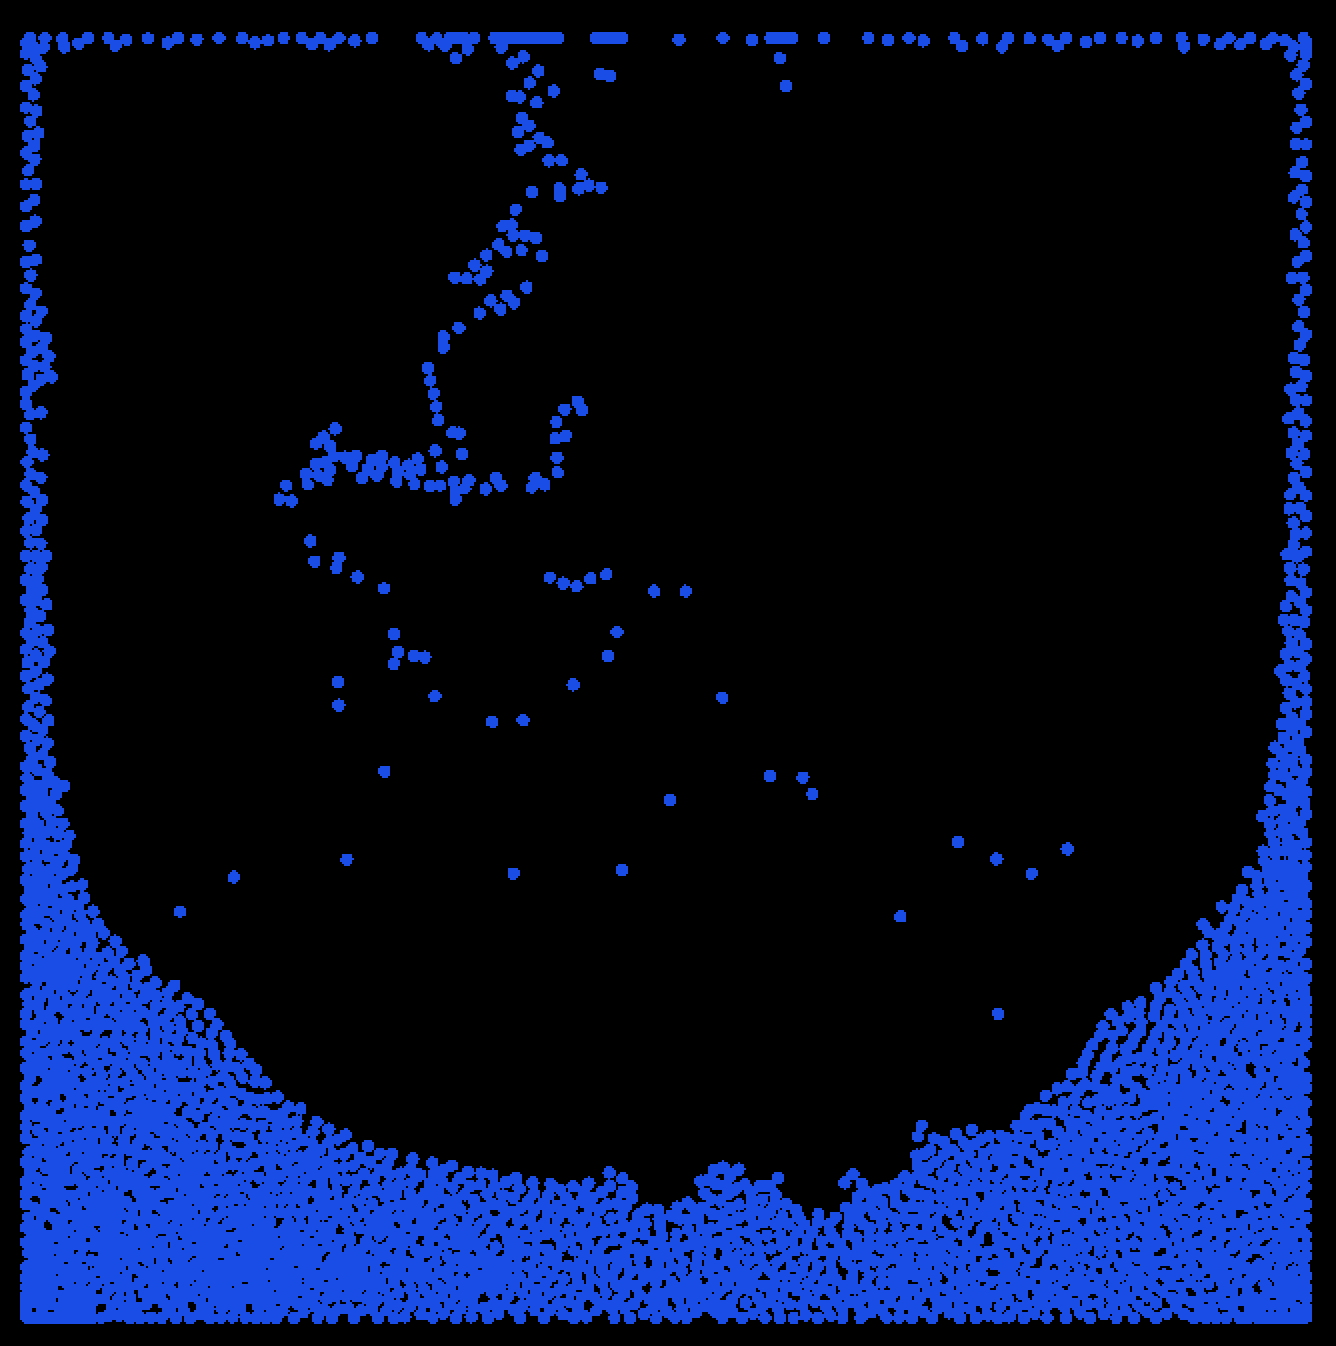
\includegraphics[width=\textwidth]{figures/apic4000.png}
        \caption{4000 particles}
    \end{subfigure}
    \hspace{1em}
    \begin{subfigure}[b]{0.2\textwidth}
        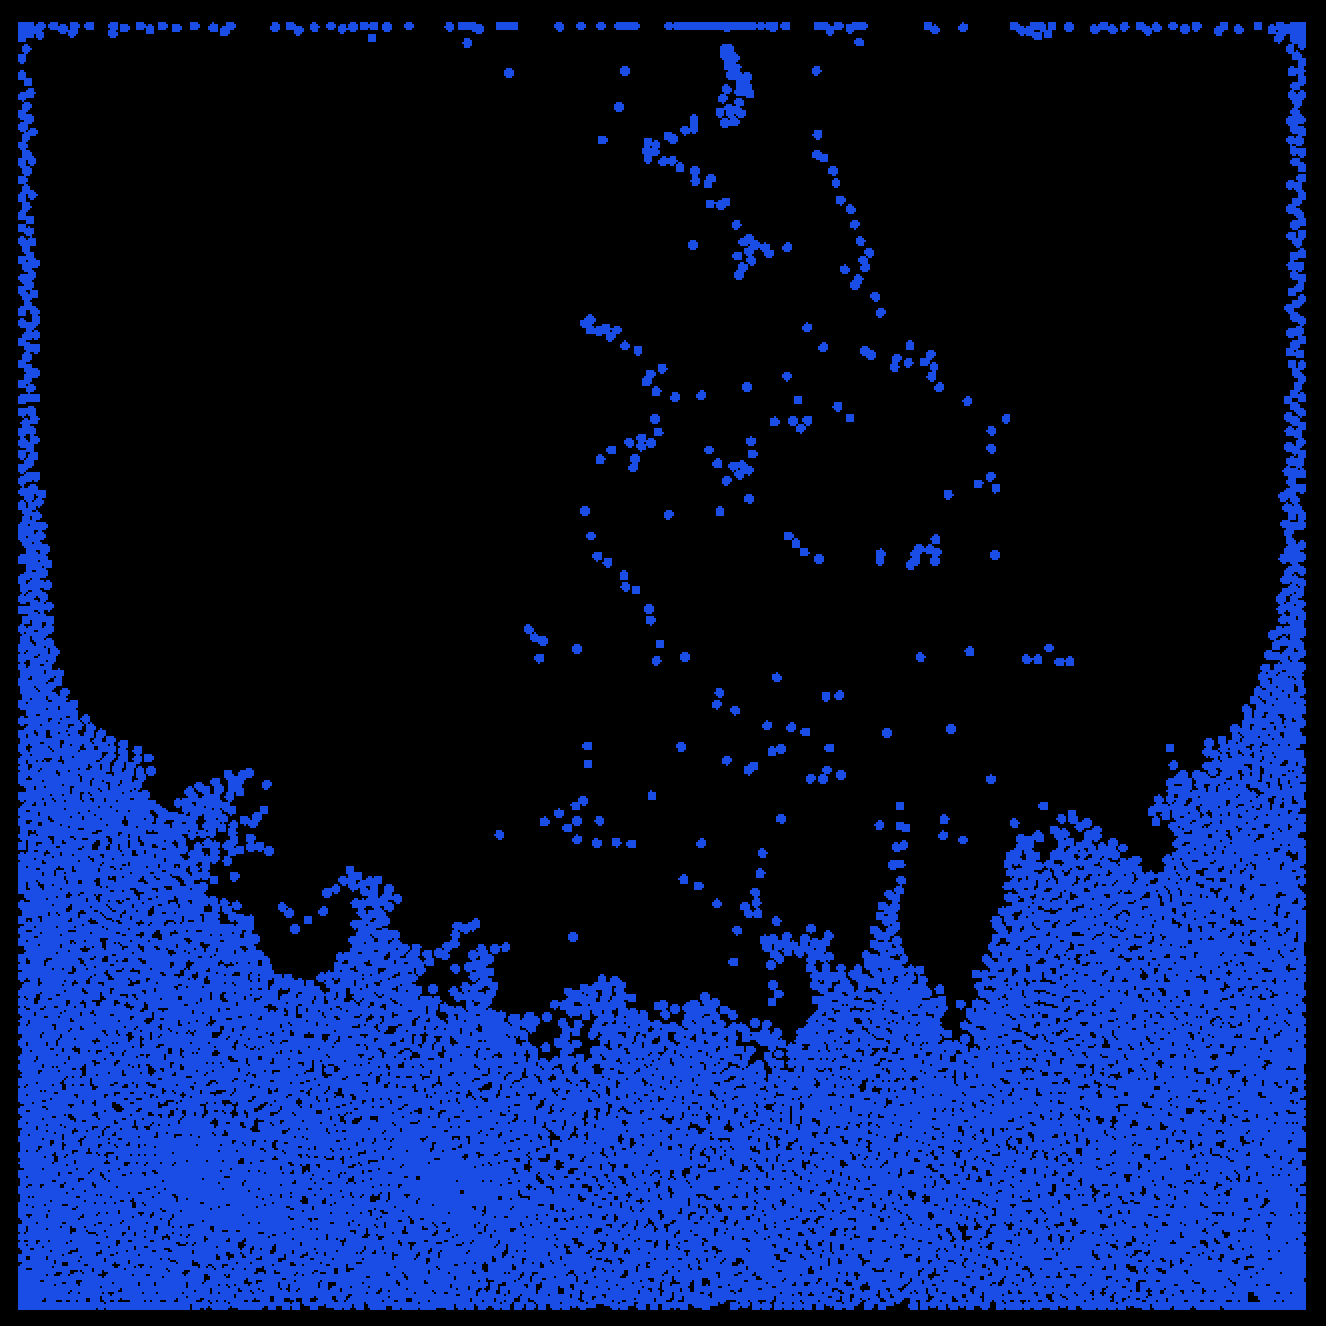
\includegraphics[width=\textwidth]{figures/apic8000.png}
        \caption{8000 particles}
    \end{subfigure}
    \caption{Comparison of APIC simulation results with increasing particle counts. 
    (a) shows the initial particle configuration, where all particles are placed in the center of the domain. 
    (b)–(d) show the simulation at the moment particles start to fall under gravity.}
    \label{fig:apic_comparison}
\end{figure*}

